\section{The multipole cutoff}
\label{sec:cutoff}

\subsection{What the cutoff is}

The vertex is built in two branches: an exact Wigner-3j sum for
$\ell\le60$, and a flat-sky Limber integral above it, truncated at
$\elmax$. The deployed value is $\elmax=1000$. The question is whether the
truncated integral has converged, and if not, what the converged answer
depends on.

Sweeping the cutoff naively answers neither, for two reasons. A partial sum
that is climbing slowly over one decade is indistinguishable from a
divergent one. And the deployed quadrature maps a fixed number of
Gauss-Legendre nodes linearly onto $[\ell_{\min},\elmax]$, so raising the
cutoff at fixed node count silently coarsens the rule and mixes truncation
with a resolution artefact.

Both are avoided by integrating in octave windows, each with its own
96-node rule. The windows are disjoint in maximum leg, so their sum is the
same integral, the node density per octave is fixed by construction, and
the partial sum up to any octave edge is the vertex built with that cutoff.
One band set therefore gives the whole curve.

\subsection{The integral converges, well above the deployed cutoff}

Table~\ref{tab:bands} gives the per-octave contribution at the source
shell, as a fraction of the total, together with the local slope $p$ from
fitting successive bands to $L^{-p}$. Positive $p$ means the tail is dying.

\begin{table}[h]
\centering
\begin{tabular}{lrrrrrr}
\toprule
& \multicolumn{3}{c}{$\gamma=0.5'$} & \multicolumn{3}{c}{$\gamma=21.9'$} \\
\cmidrule(lr){2-4}\cmidrule(lr){5-7}
band & contribution & fraction & $p$ & contribution & fraction & $p$ \\
\midrule
$(240,480]$    & $-4.19\times10^{-15}$ & 0.011 & $-3.04$ & $-1.46\times10^{-15}$ & 0.162 & $-1.89$ \\
$(480,960]$    & $-2.03\times10^{-14}$ & 0.055 & $-2.28$ & $+3.00\times10^{-16}$ & $-0.033$ & --- \\
$(960,1920]$   & $-5.57\times10^{-14}$ & 0.150 & $-1.46$ & $-1.92\times10^{-15}$ & 0.213 & --- \\
$(1920,3840]$  & $-9.69\times10^{-14}$ & 0.261 & $-0.80$ & $-2.20\times10^{-15}$ & 0.244 & $-0.20$ \\
$(3840,7680]$  & $-1.13\times10^{-13}$ & 0.303 & $-0.22$ & $-1.96\times10^{-15}$ & 0.217 & $+0.17$ \\
$(7680,15360]$ & $-8.14\times10^{-14}$ & 0.219 & $+0.47$ & $-1.49\times10^{-15}$ & 0.166 & $+0.39$ \\
\bottomrule
\end{tabular}
\caption{Octave-band contributions to $\zeta_{TTT}$ at the source shell,
tree level, on the corrected grid. The slope turns positive in the last
band at both separations, so the integral converges; it does so near
$\ell\sim10^4$, an order of magnitude above the deployed cutoff. The top
band still carries 17 to 22 percent of the total, so even $\elmax=15360$
is short of the converged value by roughly that much. Produced by
\code{code/rebuild/analyse\_cutoff.py}.}
\label{tab:bands}
\end{table}

So $\elmax$ is a numerical convergence parameter, not a physical smoothing
scale, and the deployed value of 1000 sits on the rising side of the
integrand, well below its peak. Relative to $\elmax=960$, the vertex at
$\gamma=0.5'$ on the source shell grows by

\begin{center}
\begin{tabular}{lrrrr}
\toprule
$\elmax$ & 1920 & 3840 & 7680 & 15360 \\
\midrule
tree      & 3.24 & 7.14 & 11.67 & 14.95 \\
BiHalofit & 3.26 & 7.33 & 12.90 & 18.99 \\
\bottomrule
\end{tabular}
\end{center}

\noindent
The two track each other to the first octave and then separate: by
$\elmax=15360$ the nonlinear vertex has grown by a further $27\%$ relative
to the tree one. That is the same statement as the slope table read the
other way. The nonlinear spectrum is flatter, so its turnover is later, and
its partial sum is still climbing where the tree one has begun to level
off.

The mechanism is the effective spectral slope. After the radial collapse
the hard pair contributes as a two-dimensional transverse integral
$\int\!\mathrm{d}k\,k\,P(k)$, whose integrand peaks where
$n_{\rm eff}=\mathrm{d}\ln P/\mathrm{d}\ln k$ equals $-1$ and which
converges once $n_{\rm eff}<-2$. The linear spectrum crosses $-2$ near
$k\simeq0.5\,h/$Mpc, so the tree vertex turns over at multipoles of order
$10^4$. The one-halo term flattens the nonlinear spectrum, pushing
$n_{\rm eff}$ back up to about $-1.1$ at $k\simeq1\,h/$Mpc, so the
nonlinear turnover is pushed much further out.

\subsection{The observable, as a function of the cutoff}

The vertex is not the observable. Folding each cutoff through the full
pipeline gives Table~\ref{tab:foldcut}.

\begin{table}[h]
\centering
\begin{tabular}{rrrr}
\toprule
$\elmax$ & $\xi^{\rm FK}_\kappa(0.5')$ & relative to $\elmax=960$ & as a fraction of Order-0 \\
\midrule
   960 & $+4.080\times10^{-6}$ & 1.00 & 0.48\% \\
  1920 & $+8.160\times10^{-6}$ & 2.00 & 0.97\% \\
  3840 & $+1.293\times10^{-5}$ & 3.17 & 1.53\% \\
  7680 & $+1.708\times10^{-5}$ & 4.19 & 2.02\% \\
 15360 & $+1.950\times10^{-5}$ & 4.78 & 2.31\% \\
\bottomrule
\end{tabular}
\caption{The folded FK contribution to $\xi_\kappa$ at the smallest plotted
separation, tree level, on the corrected grid, against the multipole
cutoff. Order-0 there is $8.443\times10^{-4}$. The successive factors are
$2.00$, $1.58$, $1.32$ and $1.14$, so the observable is converging, and
more quickly than the vertex does, because the fold weights the outer
shells where the vertex converges first. Extrapolating the remaining
increments puts the converged tree-level value near $2.5\%$ of Order-0. Produced by \code{code/rebuild/sweep\_cutoff.sh}
and \code{code/rebuild/fig\_cutoff.py}.}
\label{tab:foldcut}
\end{table}

This matters for how the draft's headline number should be read. The
$0.5\%$ of Order-0 that the draft quotes at arcminute separations is the
value at an unconverged cutoff. Carried to a cutoff where the integral has
turned over, the tree-level FK term is closer to $2.5\%$ of Order-0 there, a factor five above the quoted value.
The grid correction of Section~\ref{sec:sampling} and the cutoff correction
therefore push in opposite directions: the first removes the wide-angle
excess, the second raises the small-angle amplitude.

\begin{figure}[t]
\centering
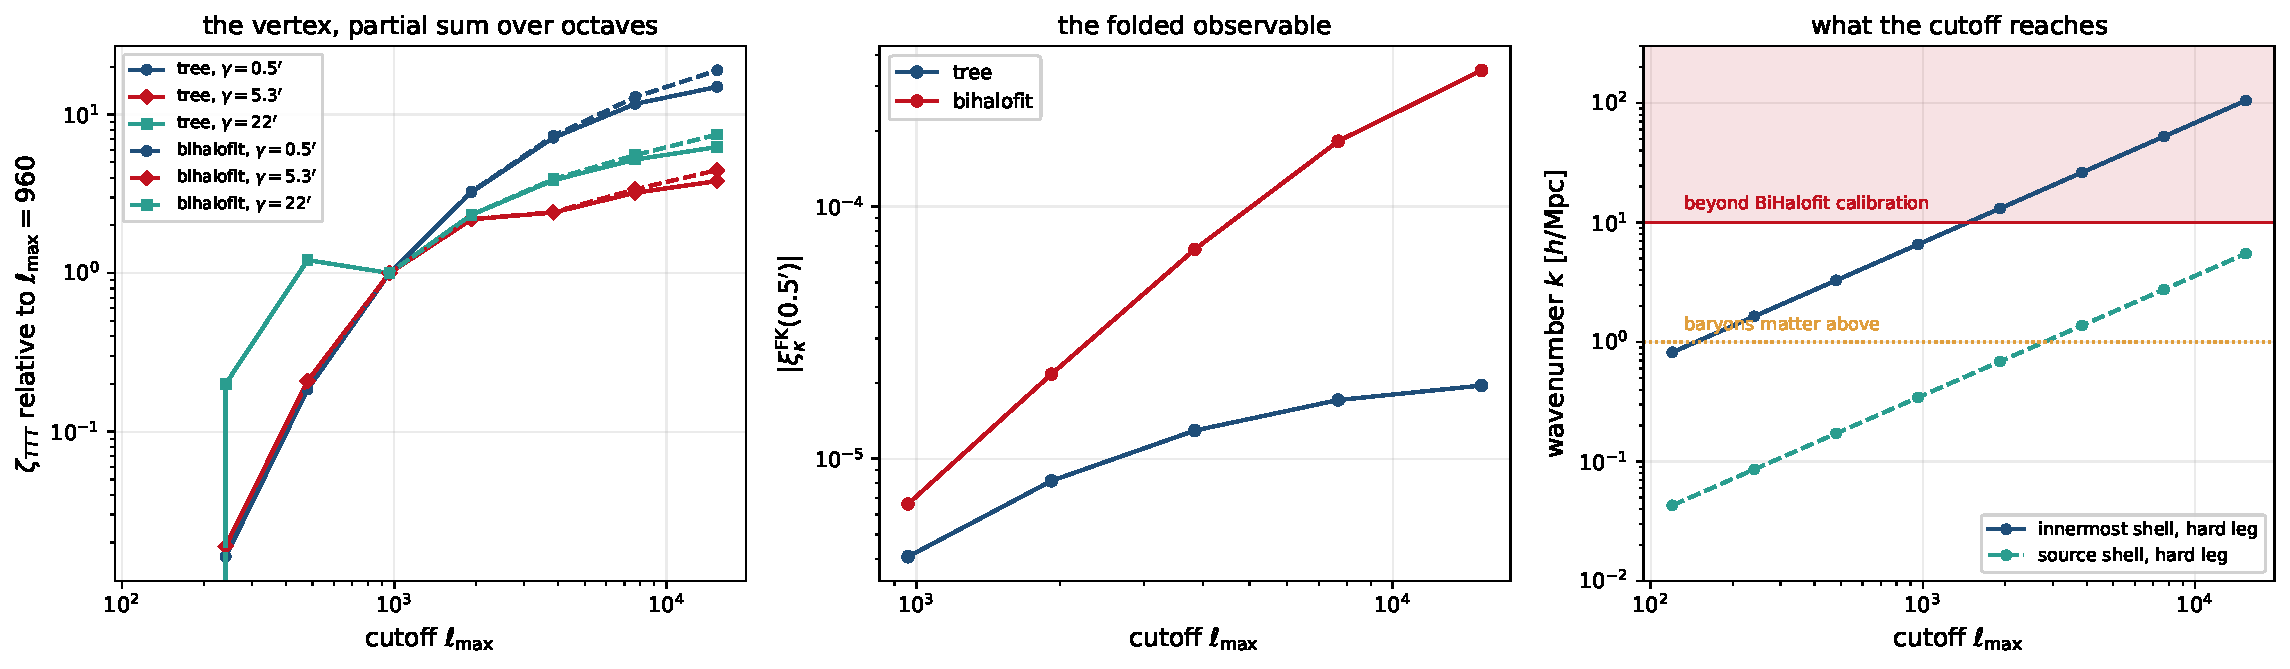
\includegraphics[width=\textwidth]{figures/cutoff_study.pdf}
\caption{Left: the vertex as a partial sum over octave windows, normalised
to the deployed cutoff. Middle: the folded observable at $\gamma=0.5'$.
Right: the wavenumber the hard leg reaches at the innermost and outermost
shells, against the range where the nonlinear bispectrum fit is calibrated
(shaded) and where baryons stop being a small correction.}
\label{fig:cutoff}
\end{figure}

\subsection{What a converged value would rest on}

This is the part that matters more than the cutoff itself. Under the Limber
branch a multipole $\ell$ at a shell of comoving distance $\chi_h$ carries
$k=\ell/\chi_h$, and the hard leg reaches $k=2\ell/\chi_h$.
Table~\ref{tab:kspace} gives both at the innermost and outermost shells.

\begin{table}[h]
\centering
\begin{tabular}{rrrrr}
\toprule
& \multicolumn{2}{c}{innermost shell, $\chi_h=293$ Mpc/$h$}
& \multicolumn{2}{c}{source shell, $\chi_h=5582$ Mpc/$h$} \\
\cmidrule(lr){2-3}\cmidrule(lr){4-5}
$\elmax$ & soft $k$ & hard $k$ & soft $k$ & hard $k$ \\
\midrule
   960 &  3.28 &   6.56 & 0.17 & 0.34 \\
  1920 &  6.56 &  13.13 & 0.34 & 0.69 \\
  3840 & 13.13 &  26.25 & 0.69 & 1.38 \\
  7680 & 26.25 &  52.50 & 1.38 & 2.75 \\
 15360 & 52.50 & 105.00 & 2.75 & 5.50 \\
\bottomrule
\end{tabular}
\caption{Wavenumbers in $h/$Mpc reached at each cutoff. BiHalofit is fitted
to simulations resolving $k\lesssim10\,h/$Mpc; baryonic feedback stops
being a small correction above $k\sim1\,h/$Mpc.}
\label{tab:kspace}
\end{table}

At the deployed cutoff the hard leg reaches $6.6\,h/$Mpc at the innermost
shell, inside the range where a nonlinear fit is calibrated. At the cutoff
where the integral has actually turned over it reaches $50$ to
$100\,h/$Mpc, which is inside single haloes: an order of magnitude beyond
BiHalofit's calibration, and a regime where baryonic physics rather than
gravity sets the matter spectrum.

The honest statement is therefore not ``the FK amplitude is $X$''. It is
that the tree-level FK amplitude converges by $\elmax$ of order $10^4$, and
that a converged \emph{nonlinear} FK amplitude is a statement about the
one-halo regime rather than about the bispectrum physics the draft
describes. Reporting the amplitude as a function of the small-scale cutoff
is the defensible presentation.

\subsection{A practical ceiling}

The Limber branch evaluates the hard leg at $k=2\elmax/\chi_h$, and the
fiducial $P(k)$ table stops at $k_{\max}=206\,h/$Mpc, with no
extrapolation. At the innermost deployed shell, $\chi_h=293$ Mpc/$h$, that
caps the reachable cutoff at $\elmax=k_{\max}\chi_h/2\simeq30\,000$. The
cutoffs used here stay inside that. Pushing further needs a longer $P(k)$
table, and the same relation read the other way is the structural floor on
the smallest usable shell discussed in Section~\ref{sec:lambdamin}.
